\documentclass[a4paper, 12pt]{article}
\usepackage[utf8]{inputenc}
\usepackage{graphicx}
\graphicspath{ {images/} }
\usepackage[a4paper,left=1.5in,right=1in,top=1in,bottom=1in]{geometry}
\usepackage{tikz}
\usetikzlibrary{positioning,shapes,fit,arrows}
\definecolor{myblue}{RGB}{56,94,141}
\usepackage{fancyhdr}
\usepackage{booktabs}
\usepackage{mathtools}
\usepackage{amsmath}
\usepackage{etoolbox}
%\apptocmd{\thebibliography}{\csname phantomsection \endcsname \addtocontentsline{toc}{chapter}{\bibname}}{}{}
\usepackage{caption}
\usepackage{float}
\restylefloat{figure}
\pagestyle{fancy}
\fancyhf{}
\fancyfoot[CE,CO]{ \raggedright{P:F-SMR-UG/08/R0} }
\fancyfoot[LE,RO]{\thepage}
\renewcommand{\headrulewidth}{0pt} 

\begin{document}
\begin{titlepage}
\hspace{15pt}
\begin{center}
\textbf{{\Large A Project Based Seminar Report}}
\end{center}

\begin{center}
On
\end{center}

\begin{center}
{\fontsize{18pt}{21.6pt}\selectfont \textbf{\textcolor[HTML]{FF0000}{$``$Indoor Navigation System$"$ }}}
\end{center}

\begin{center}
Submitted to the
\end{center}

\begin{center}
{\large Savitribai Phule Pune University }
\end{center}

\begin{center}
In partial fulfillment for the award of the Degree of
\end{center}

\begin{center}
{\large Bachelor of Engineering }
\end{center}

\begin{center}
In
\end{center}

\begin{center}
{\large Information Technology}
\end{center}

\begin{center}
By
\end{center}

\begin{center}
{\fontsize{16pt}{19.2pt}\selectfont \textbf{\textcolor[HTML]{FF0000}{Manvi Pandya}}\par}
\end{center}

\begin{center}
\textcolor[HTML]{FF0000}{(71828960)}
\end{center}

\begin{center}
Under the guidance of
\end{center}

\begin{center}
{\fontsize{16pt}{19.2pt}\selectfont \textbf{\textcolor[HTML]{FF0000}{\Large Prof. R. R. Chhajed}}\par}
\end{center}
\vspace{\baselineskip}
\begin{figure}[H]
    \centering
		
\includegraphics[width=1.84in,height=1.84in]{Pict_logo.png}
\end{figure}
\begin{center}
{\large Department Of Information Technology}
\end{center}

\begin{center}
{\Large Pune Institute of Computer Technology College of Engineering}
\end{center}

\begin{center}
Sr. No 27, Pune-Satara Road, Dhankawadi, Pune - 411 043.\textbf{ }
\end{center}

\begin{center}
\textbf{{\Large 2019-2020}}
\end{center}
\end{titlepage}
\pagebreak
%2
\begin{titlepage}
\begin{figure}[H]
    \centering
		
\includegraphics[width=1.84in,height=1.84in]{Pict_logo.png}
\end{figure}
\begin{center}
\textbf{{\LARGE CERTIFICATE}}
\end{center}

This is to certify that the project based seminar report entitled
\textbf{\textcolor[HTML]{FF0000}{$``$Indoor Navigation System$"$ }} being submitted by \textbf{\textcolor[HTML]{FF0000}{Manvi Pandya  (71828960)}} is a record as bonafide work carried out by him/her under the supervision and guidance of \textbf{\textcolor[HTML]{FF0000}{Prof. R. R. Chhajed}} in partial fulfillment
of the requirement for \textbf{TE (Information Technology Engineering) -- 2015 
course} of Savitribai Phule Pune University, Pune in the academic year 2019-20.
\linebreak
\linebreak
\linebreak
\linebreak
\linebreak
\linebreak
\linebreak
\linebreak
\linebreak
Date:\hspace{15pt} /\hspace{15pt}/2020\hspace{400pt}
\linebreak
\linebreak
Place:\hspace{15pt}Pune\hspace{15pt}\hspace{15pt}\hspace{15pt}\hspace{15pt}\hspace{15pt}\hspace{15pt}\hspace{15pt}\hspace{15pt}
\linebreak
\linebreak
\textcolor[HTML]{FF0000}{Prof. R. R. Chhajed}\hspace{200pt}\textcolor[HTML]{FF0000}{Dr. A.M.Bagade}

\hspace{20pt}Guide\hspace{220pt}Head of the Department

\begin{center}\textcolor[HTML]{FF0000}{Dr.  P. T. Kulkarni}\end{center}
\begin{center}
Principal
\end{center}
\begin{center}
\line(1,0){465}
\end{center}
{\large This Project Based Seminar report has been examined by us as per the
Savitribai Phule Pune University, Pune requirements at \textcolor[HTML]{FF0000}{Pune Institute of Computer Technology, Pune - 411043} on ............................. }
\linebreak
\linebreak
\linebreak
\linebreak
\linebreak
\linebreak
{\raggedright
{\large Internal Examiner \hspace{170pt}External Examiner}
}
\end{titlepage} 
\newpage
\pagenumbering{Roman}
\begin{center}
    I
\end{center}
\begin{center}
    \section*{ACKNOWLEDGEMENT}
\end{center}
\hspace{0.5cm}Our project based seminar would not have been possible without the kind support and help of many individuals and our organization. I would like to extend my sincere thanks to all of them.
\vspace{0.25cm}
\par I am feeling obliged in taking the opportunity to sincerely thank Prof. R. R. Chhajed, our seminar guide, for her guidance and without whose help and support throughout, this seminar would not have been possible. I am highly indebted to Prof. Manish Khodaskar for their guidance and constant supervision as well as for providing necessary information regarding the seminar and also for their support in completing the seminar.
\vspace{0.25cm}
\par I would like to express my gratitude towards Dr. A.M. Bagade, Head of Information Technology Department, for their kind cooperation and encouragement to present our ideas through this seminar. My thanks and appreciations also go to my seminar group members in developing the seminar and co-operating throughout the working process.
\vspace{0.25cm}
\par Last but not the least I also would like to thank my family and friends to keep me motivated to complete this seminar.

\newpage
\begin{center}
    II
\end{center}
\begin{center}
    \section*{Abstract}
\end{center}
Today the navigation systems are highly accurate with help of Global Positioning System (GPS) for outdoor navigation process. However, the lack of GPS signal reception inside the buildings makes indoor navigation process an interesting challenge. Most systems that have been developed so far lack the adaptability to changes that our system provides to the user. 
\par 
The idea presents the design of an indoor space representation technique and an interface that will provide navigation feature for that indoor environment using a WebApp. The user is alerted with a link that directs him to our WebApp as soon as he enters the zone. Here, the user’s role is to enter start and end location and the application provides the user with the optimized path. To find the shortest path Dijkstra’s or A* algorithms will be used. For the implementation purpose Bluetooth Low Energy(BLE), iBeacons will be used. These devices emit continuous radio packets and were conventionally modelled for advertisements, and these signals can be used for positioning. 
\par
All that a user need is a smartphone. This system will be used especially in big industries, offices, shopping mall or college campus.
\linebreak
\section*{Keywords}
Indoor navigation; iBeacons; A* or Dijkstra’s algorithm; GPS; BLE.
\newpage
\begin{center}
    III
\end{center}
\begin{center}
    \section*{Abreviations}
\end{center}

{\raggedright
\vspace{3pt} \noindent \begin{tabular}{|p{100pt}|p{167pt}|p{148pt}|}
\hline
\parbox{100pt}{\centering \textbf{Sr. No.}} & 
\parbox{167pt}{\centering \textbf{Abbreviations}} & 
\parbox{148pt}{\centering \textbf{Full form}} \\
\hline
\parbox{100pt}{\centering 1} & 
\parbox{167pt}{\centering GPS} & 
\parbox{148pt}{\centering Global Positioning System} \\
\hline
\parbox{100pt}{\centering 2} & 
\parbox{167pt}{\centering BLE} & 
\parbox{148pt}{\centering Bluetooth Low Energy} \\
\hline
\parbox{100pt}{\centering 3} & 
\parbox{167pt}{\centering IPS} & 
\parbox{148pt}{\centering Indoor Positioning System} \\
\hline
\parbox{100pt}{\centering 4} & 
\parbox{167pt}{\centering GPSL} & 
\parbox{148pt}{\centering Google Play Services Location} \\
\hline
\parbox{100pt}{\centering 5} & 
\parbox{167pt}{\centering RSSI} & 
\parbox{148pt}{\centering Received Signal Strength indication} \\
\hline
\parbox{100pt}{\centering 6} & 
\parbox{167pt}{\centering PDR} & 
\parbox{148pt}{\centering Pedestrian Dead Reckoning} \\
\hline
\parbox{100pt}{\centering 7} & 
\parbox{167pt}{\centering MAC} & 
\parbox{148pt}{\centering Media access control} \\
\hline


\end{tabular}
\vspace{2pt}

}
\newpage
\begin{center}
    IV
\end{center}
{\raggedright Acknowledgement\hspace{320pt}I}
\linebreak
{\raggedright Abstract\hspace{367pt}II}
\linebreak
{\raggedright Abbreviations\hspace{340pt}III}
\linebreak
{\raggedright Contents\hspace{365pt}IV}
\linebreak
{\raggedright List of Tables\hspace{343pt}V}
\linebreak
{\raggedright List of Figures\hspace{338pt}VI}
\linebreak
\tableofcontents
\newpage
\begin{center}
    V
\end{center}


\begin{center}
\textbf{{\Large LIST OF TABLES}}
\end{center}

\begin{table}[h!]
    \centering
    \begin{tabular}{|c|l|c|}
    \hline
    Sr. No.& Table Name & Page No. \\
    \hline
    1 & Summary of other papers & 9\\
    \hline
    \end{tabular}
    \caption*{}
    \label{tab:my_label2}
\end{table}
\par
\newpage
\begin{center}
    VI
\end{center}

\begin{center}
\textbf{{\Large LIST OF FIGURES}}
\end{center}

\begin{table}[h!]
    \centering
    \begin{tabular}{|c|l|c|}
    \hline
    Sr. No.& Figure Name & Page No. \\
    \hline
1 & Technology stack & 11 \\
2 & Workflow & 13 \\
\hline

    \end{tabular}
    \caption*{}
    \label{tab:my_label2}
\end{table}

\newpage


\pagenumbering{arabic}
\begin{center}
\section{INTRODUCTION}
\end{center}
\subsection{Introduction to Indoor Navigation System}
\par
An indoor navigation system is a system that provides navigation within buildings. Nowadays, the majority of people use the Global Positioning System (GPS) for outdoor navigation processes. However, the lack of GPS signal reception inside the buildings cannot provide accurate navigation within a building and that is where an indoor positioning system (IPS) comes in. An indoor positioning system acts as a GPS, but specifically for buildings.
 \\ 
\subsection{Motivation behind project topic} 
\par
This project is motivated by the following challenges which we do not believe can be addressed by current approaches . It includes locating gate ,check-in counters at airports ,Helping patients find labs/doctors rooms ,Providing shortest path for patients and doctors during emergency situations ,Identifying location of all forklifts in the warehouse on a real-time basis,Remembering parking lot,locating and navigating to conference rooms in an enterprise,Helping with emergency exit during crisis and so many more.
\\
\subsection{Aim and Objective(s) of the work} 
\par Infrastructure items, such as hosts, can be broken into by a competing company to attain confidential information about its users and other data that is stored on the machine. This in turn allows workflows to be changed, i.e. by breaking in a system and patching the code-base or the platform itself, or simply by reverse engineering workflows and creating rogue clients.
\\
\par
Objective is to detect the position of the user automatically when in online mode ,to provide an application which will guide the user inside the building and show their progress while they navigate ,to provide the user with the shortest path to reach to the destination along with all the feasible paths ,to provide an admin panel to the owner of the premises, in order to enter the floorplan of the location and is also responsible for plotting points of features and possible paths,to help the user locate their friends if they are nearby/in the same building (Find a friend) and to provide users with paths to emergency exit in case of an emergency.
\\
\subsection{Introduction to Positioning Techniques	}
\par 
Positioning techniques is the most important aspect of the project. As the application’s main aim is to detect the position of the user and provide appropriate path to the user. There are various positioning techniques used for the detection of the user’s position. There is a requirement of a technique which is accurate, easy to install and which can be used by the user very easily.
\\
\newpage

\begin{center}

\section{LITERATURE SURVEY}

\end{center}



\subsection{An Indoor Positioning and Navigation Application for Visually Impaired People using Public Transport}
\hspace{1cm}This paper describes the results of a project setup at NAWI Graz Graz University of Technology Graz, Austria  and was an indoor positioning and indoor navigation system for use in public transport systems, and especially for use by visually impaired people.An application was developed for outdoor indoor positioning and navigation between different modes and vehicles. It allows the user to request a navigation route and to compute all possible transportation routes for all available modes of transport.
\par Positioning is graph-based PDR approach that uses the tactile paths, is used with Bluetooth Low Energy (BLE) beacons, and combined with the default location provided by the smartphone(For Android devices, this default location is provided via Google Play Services ).It requires three estimations including:Attitude Estimation , Graph-based PDR and Bluetooth Combination and Positioning service 
In Navigation ,Given start and target nodes, the shortest path is computed using Dijkstra’s algorithm.
\\
\linebreak
\textbf{ADVANTAGES}
\begin{enumerate}
	\item It was made for both indoor and outdoor navigation and automatically switches between technologies (GPSL or beacons).
	\item	Since it was made specially for blind people,its results are accurate. 
	\item	No additional infrastructure was installed and no additional electricity was used, an indoor positioning system was created that operates independent of additional infrastructure.
	\item Voice Navigation feature is present.
	
\end{enumerate}

\textbf{DISADVANTAGES:}
\begin{enumerate}
	\item No admin panel.
	\item Since it focuses more on accuracy it is very slow and thus can not be used by the general public.
	\item It requires a tactile path, which is not there in developing countries like india.
	\item A malfunction of the algorithm was observed if the smartphone flipped over .
	\item Application is required to be installed (So users unaware of the app can not use it).
	\item  Application is only in regional language(German) which makes it difficult for people from outside to use the service.	
\end{enumerate}
\textbf{This paper focuses more on accuracy than efficiency and is thus not useful for the general public who are visually paired where lack in accuracy will be  managed (by a few meters) but optimised solution is required.}


\subsection{A Smart Indoor Navigation System over BLE}
\hspace{1cm}  
The proposed indoor navigation system is launched on the third floor, building 8, Faculty of Engineering, Cairo University In this paper, a smart indoor navigation system over BLE is demonstrated. It uses a Raspberry Pi board as a scanner. While using iBeacons for floor planning the scanned area. Then navigation is based on A* algorithm. Finally, a low-power consumption is achieved usingiBeacons with a good navigation accuracy using A* algorithm.Working Include 3 steps as follows:
\begin{itemize}
	\item	Trilateration: Trilateration uses the distances from each of the known locations to determine the coordinate of the unknown location .
	\item Particle Filter: The particle filter is a way of implementing the recursive Bayesian filter(compute estimates based on random samples). 
	\item	A* Algorithm: A* algorithm is an extension of the Dijkstra’s algorithm.	
\end{itemize}
\textbf{Hardware used were Bluetooth Low Energy(BLE) , Estimote Beacons ,RaspberryPi.}
\linebreak
\textbf{Software used were Backend(LAMP Platform) , Frontend(Web page).}
\textbf{ADVANTAGES}
\begin{enumerate}
	\item	It provides positioning with low power requirements.
	\item	It provides high accuracy by using A* algorithm.
	\item	User-friendly Interface.
	\item  Use of LAMP platform make it platform independent.	
\end{enumerate}
\textbf{DISADVANTAGES}
\begin{enumerate}
	\item	For positioning it uses triangulation method which is not very accurate so to increase it’s accuracy particle filters are used which add up to the cost and complexities.
	\item	No Admin Panel .
	\item It was designed for single floor.
	\item Application is required to be installed (So users unaware of the app can not use it).
	\item	No additional features for users.		
\end{enumerate}
\textbf{This paper provides high accuracy in positioning using Beacons and optimised navigation using A* algorithm which gives much better results than previous discussed technologies.But positioning using triangulation can be improved by using some different computation which further reduces need of particle filters.}
\subsection{Improved indoor position estimation algorithm based on geo-magnetism }
\hspace{1cm} 
In this paper , Positioning is based on the geomagnetic field . Most of the similar projects make use of particle filters .The particle filter improved the accuracy of location positioning. However,calculation cost can be high for multiple particles and can take longer time to estimate the accurate locations of users.Users also need to move a certain distance before determining their locations.  In this paper, they introduced an algorithm that can decrease processing loads of the particle filter and can detect user locations more quickly\\
\par The experiment took place on the third floor of the electronic building of Yeungnam University The corridor was square-shaped, 67m wide, and 12m tall. The surroundings included spaces such as lab, office, and library.
\\
Positioning includes 4 steps as follows:
\begin{itemize}
	\item Measurement step, measures magnetic intensity of the current location using the magnetometer. 
	\item	Prediction step,  generates N number of particles which are calculated for weight values via prior probability of previously generated particles with a number N.
	\item	Weight update step, Gaussian density function is used for updating weight values.
	\item	Resampling step, with a probability proportional to the weight value  particles that are to be included in the new particle group 		
\end{itemize}
NN algorithm, pre-existing particle filter, and modified particle filter all three are implemented.
\linebreak
\linebreak
RESULT
\begin{itemize}
	\item Particles are generated only in a few candidate locations using Euclidean distance. 
	\item	Since few particles are generated for weight value calculation, there are fewer numbers of particles that consume processing power causing less overhead issues. 
	\item Locations can be estimated more quickly. 	
\end{itemize}
\textbf{ADVANTAGES}
\begin{enumerate}
	\item	High Accuracy is achieved with particle filter in less amount and time.
	\item	Geomagnetic field removes the need for additional infrastructure.
	\item	Algorithm introduced showed better results than previous results.
	
\end{enumerate}
\textbf{DISADVANTAGES}
\begin{enumerate}
	\item	Using Particle Filter is still costly and complex.
	\item	It is suitable for ideal situations only(no noise or disturbances).
	\item	Real-time use is very difficult.
	\item	No Admin Panel
	\item	No additional features		
\end{enumerate}
\textbf{This method provides accuracy but for a smaller and already known area which do not have much disturbances and noise which is practically not possible with any public place .Thus implementation in real-time scenario is not possible .}
\newpage

\begin{center}
	\text{Table no. 1 Summary of other papers}
\end{center}

\vspace{3pt} \noindent
\begin{tabular}{|p{107pt}|p{107pt}|p{107pt}|p{107pt}|}
	\hline
	\parbox{107pt}{\raggedright Topic} & 
	\parbox{107pt}{\raggedright } & \parbox{107pt}{\raggedright Advantages} & \parbox{107pt}{\raggedright Disadvantages} \\
	\hline
	\parbox{107pt}{\raggedright Time-Efficient Indoor Navigation and Evacuation With Fastest Path Planning Based on Internet of Things Technologies} &
	\parbox{107pt}{\raggedright 2019 IEEE TRANSACTIONS ON SYSTEMS, MAN, AND CYBERNETICS: SYSTEMS} & 
	\parbox{107pt}{\raggedright 
		\begin{enumerate}
			\item Finds the fastest path and shortest path based on congestion
			\item In case of emergency, provides closest exit without congestion
			\item Friend's location can be detected
	\end{enumerate}} & 
	\parbox{107pt}{\raggedright No admin panel} \\
	\hline
	\parbox{107pt}{\raggedright Mobile Indoor Navigation System in iOS Platform Using Augmented Reality} & 
	\parbox{107pt}{\raggedright } & 
	\parbox{107pt}{\raggedright Augmented reality is more accurate} & \parbox{107pt}{\raggedright 
		\begin{enumerate}
			\item Starting point should be entered manually
			\item Not feasible in new places
			\item For accuracy purpose, gender and height is required of user (user specific)
	\end{enumerate}} \\
	\hline
	\parbox{107pt}{\raggedright Indoor Navigation System using BLE Beacons} & 
	\parbox{107pt}{\raggedright 2019 International Conference on Nascent Technologies in Engineering (ICNTE 2019)} & 
	\parbox{107pt}{\raggedright 
		\begin{enumerate}
			\item Uses web app rather than traditional apps
			\item Has admin panel
			\item Dynamic interaction and adaptability to changes
	\end{enumerate}} & 
	\parbox{107pt}{\raggedright 
		\begin{enumerate}
			\item Need internet connection
			\item Fastest path is not provided
	\end{enumerate}} \\
	\hline
\end{tabular}

\pagebreak

\vspace{3pt} \noindent
\begin{tabular}{|p{107pt}|p{107pt}|p{107pt}|p{107pt}|}
	\hline
	\parbox{107pt}{\raggedright Topic} & 
	\parbox{107pt}{\raggedright } & \parbox{107pt}{\raggedright Advantages} & \parbox{107pt}{\raggedright Disadvantages} \\
	\hline
	\parbox{107pt}{\raggedright An Indoor Positioning and Navigation Application for Visually Impaired People using Public Transport} & 
	\parbox{107pt}{\raggedright 2018 International Conference on Indoor Positioning and Indoor Navigation (IPIN), 24-27 September 2018, Nantes, France} & 
	\parbox{107pt}{\raggedright 
		\begin{enumerate}
			\item Both outdoor(GPS) and indoor(PDR) navigation system
			\item Different modes are also shown including railway (Graz main railway station) to reach target point
	\end{enumerate}} & 
	\parbox{107pt}{\raggedright 
		\begin{enumerate}
			\item Uses PDR algorithm which is very complex
			\item PDR is not accurate as beacons
			\item Uses tactile paths which is difficult to follow
			\item Useful only for visually impaired people
		\end{enumerate}
	} \\
	\hline
	\parbox{107pt}{\raggedright Smart Indoor Navigation System over BLE} &
	\parbox{107pt}{\raggedright 2019 8th International Conference on Modern Circuits and Systems Technologies (MOCAST)} & 
	\parbox{107pt}{\raggedright 
		\begin{enumerate}
			\item A* algorithm
			\item Beacon (accuracy upto 1m)
		\end{enumerate}
	} & \parbox{107pt}{\raggedright 
		\begin{enumerate}
			\item Need internet connection
			\item No admin panel (Blueprint is a pre-requisite)
	\end{enumerate}} \\
	\hline
	\parbox{107pt}{\raggedright Indoor pedestrian navigation algorithm based on smartphone mode recognition} & 
	\parbox{107pt}{\raggedright 2019 IEEE 3rd Information Technology, Networking, Electronic and Automation Control Conference (ITNEC 2019)} & 
	\parbox{107pt}{\raggedright 
		\begin{enumerate}
			\item Neural networks are used (accuracy 99.45\%)
			\item Heading correction method is used
			\item Step length method is used to improve accuracy
	\end{enumerate}} & 
	\parbox{107pt}{\raggedright Inertial sensors are required for positioning which is not practically possible (first aspect)} \\
	\hline
\end{tabular}
\vspace{2pt}

\pagebreak

\vspace{3pt} \noindent
\begin{tabular}{|p{107pt}|p{107pt}|p{107pt}|p{107pt}|}
	\hline
	\parbox{107pt}{\raggedright Topic} & 
	\parbox{107pt}{\raggedright } & \parbox{107pt}{\raggedright Advantages} & \parbox{107pt}{\raggedright Disadvantages} \\
	\hline
	\parbox{107pt}{\raggedright Using A* algorithm to find shortest path in Indoor positioning system} & 
	\parbox{107pt}{\raggedright 2017,International Research Journal of Engineering and Technology (IRJET), June -2017} & 
	\parbox{107pt}{\raggedright 
		\begin{enumerate}
			\item A* gives a faster and efficient result.
			\item A* uses heuristic to achieve better performance.
	\end{enumerate}} & 
	\parbox{107pt}{\raggedright A* algorithm is hard to apply on 3D floor plan so 2D plan was used.} \\
	\hline
	\parbox{107pt}{\raggedright BLE Beacons for Internet of Things Applications: Survey, Challenges and Opportunities} & 
	\parbox{107pt}{\raggedright IEEE Internet of Things Journal, Vol. A, No. B, Month 2018} & 
	\parbox{107pt}{\raggedright 
		\begin{enumerate}
			\item Beacons have more accuracy than GPS.
			\item Advertising is done using beacons which is of great use.
	\end{enumerate}} & 
	\parbox{107pt}{\raggedright 
		\begin{enumerate}
			\item Beacons' batteries are need to be changes after almost every 5 to 8 years.
			\item Also, there are some security issues with beacons.
		\end{enumerate}
	} \\
	\hline
	\parbox{107pt}{\raggedright Application of Augmented Reality in Campus Navigation} & 
	\parbox{107pt}{\raggedright International Conference on Precision Machining, Non-Traditional Machining and Intelligent Manufacturing, 2019} &
	\parbox{107pt}{\raggedright 
		\begin{enumerate}
			\item It is a less time consuming process
			\item Improved framework so that more users interacted in a synchronize manner.
	\end{enumerate}} & 
	\parbox{107pt}{\raggedright 
		\begin{enumerate}
			\item It is very expensive to implement and develop.
			\item Lack of security in as issue.
			\item Low performance level.
		\end{enumerate}
	} \\
	\hline
	\parbox{107pt}{\raggedright A Survey of Positioning Systems Using Visible LED Lights} & 
	\parbox{107pt}{\raggedright IEEE Communications Surveys and Tutorials, Vol. 20, No. 3, Third Quarter 2018} & 
	\parbox{107pt}{\raggedright 
		\begin{enumerate}
			\item It is easy to install.
			\item It is not affected with Radio Frequency systems
		\end{enumerate}
	} & \parbox{107pt}{\raggedright 
		\begin{enumerate}
			\item Data decoding is difficult.
			\item It has low accuracy for positioning in corners or edges.
	\end{enumerate}} \\
	\hline
\end{tabular}
\vspace{2pt}

\pagebreak

\vspace{3pt} \noindent
\begin{tabular}{|p{107pt}|p{107pt}|p{107pt}|p{107pt}|}
	\hline
	\parbox{107pt}{\raggedright Topic} & 
	\parbox{107pt}{\raggedright } & \parbox{107pt}{\raggedright Advantages} & \parbox{107pt}{\raggedright Disadvantages} \\
	\hline
	\parbox{107pt}{\raggedright Improved indoor position estimation algorithm based on geo-magnetism intensity } & 
	\parbox{107pt}{\raggedright 2018 International Conference on Indoor Positioning and Indoor Navigation, 27th-30th October 2018} & 
	\parbox{107pt}{\raggedright 
		\begin{enumerate}
			\item High Accuracy is achieved with particle filter in less amount and time.
			\item Geomagnetic field removes the need of additional infrastructure.
			\item Algorithm introduced showed better results than previous results.
	\end{enumerate}} & 
	\parbox{107pt}{\raggedright 
		\begin{enumerate}
			\item Using Particle Filter is still costly and complex.
			\item It is suitable for ideal situations only(no noise or disturbances).
			\item Real-time use is very difficult.
			\item No Admin Panel
			\item No additional features
	\end{enumerate}} \\
	\hline
	\parbox{107pt}{\raggedright Indoor Navigation Using A* Algorithm} & \parbox{107pt}{\raggedright 2016,Springer International Publishing AG 2017 T. Herawan et al. (eds.)} & 
	\parbox{107pt}{\raggedright 
		\begin{enumerate}
			\item This application uses A* algorithm which is more efficient than Dijkstra.
			\item The application displays the user’s progress along the route and issues instructions for each turn.
	\end{enumerate}} & 
	\parbox{107pt}{\raggedright 
		\begin{enumerate}
			\item The application is unable to locate the user; it can only know which floor the user currently locates through the input by the user.
			\item The application only provides navigation in two-dimension (2D).
		\end{enumerate}
	} \\
	\hline
\end{tabular}
\vspace{2pt}

\pagebreak

\vspace{3pt} \noindent
\begin{tabular}{|p{107pt}|p{107pt}|p{107pt}|p{107pt}|}
	\hline
	\parbox{107pt}{\raggedright Topic} & 
	\parbox{107pt}{\raggedright } & \parbox{107pt}{\raggedright Advantages} & \parbox{107pt}{\raggedright Disadvantages} \\
	\hline
	\parbox{107pt}{\raggedright } &
	\parbox{107pt}{\raggedright } &
	\parbox{107pt}{\raggedright } &
	\parbox{107pt}{\raggedright 
		\begin{enumerate}
			\setcounter{enumi}{2}
			\item The floor plan shown in the application cannot be zoom in or zoom out.
			\item A* algorithm is hard to apply on 3D floor plan so 2D plan was used.
	\end{enumerate}} \\
	\hline
	\parbox{107pt}{\raggedright Indoor Navigation based on Linked Data at Honvéd Hospital, Budapest} & 
	\parbox{107pt}{\raggedright 2018,IEEE 12th International Symposium on Applied Computational Intelligence and Informatics.} & 
	\parbox{107pt}{\raggedright 
		\begin{enumerate}
			\item The Linked Open Data technology is a form of the Semantic Web which exploits the advantages of data on the internet.
			\item RDF is designed to store information in a flexible fashion
	\end{enumerate}} & 
	\parbox{107pt}{\raggedright 
		\begin{enumerate}
			\item The challenge during the development was to migrate the data from RDF datatype into Neo4j database.
			\item RDF database exposed some limitations considering the shortest path algorithm.
			\item Neo4j is optimized for graph traversals and finding the shortest paths and spanning trees which is the disadvantage of Neo4j over RDF.
	\end{enumerate}} \\
	\hline
\end{tabular}
\vspace{2pt}
\newpage
\begin{center}
\section{ABOUT PROJECT}
\end{center}
\subsection{TECHNOLOGY STACK}
\begin{figure}[h!]
    \centering
    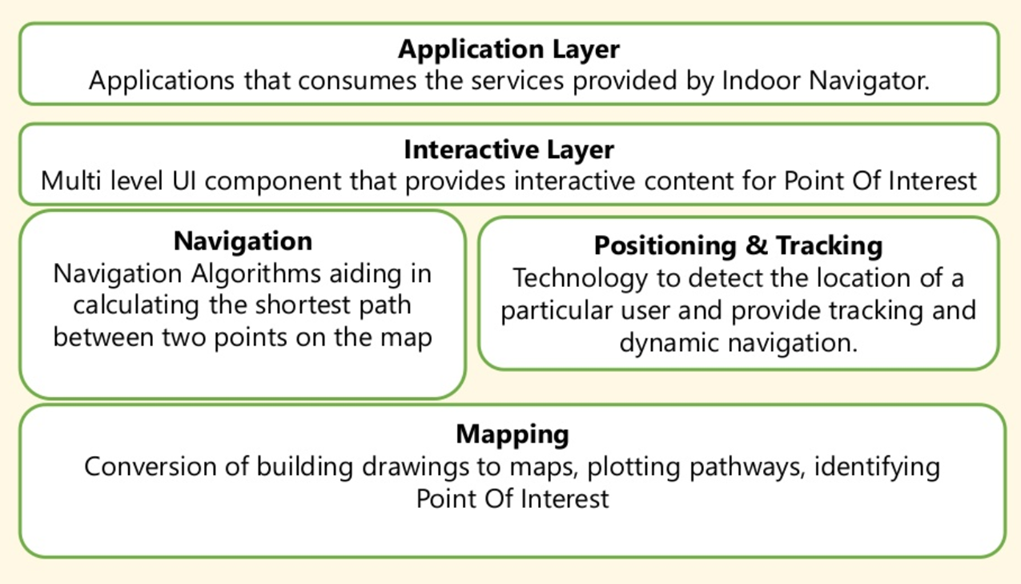
\includegraphics[width = 6in]{1.png}
    \caption{Technology stack}
    \label{fig: blockbit}
\end{figure}
\begin{enumerate}
 \item \textbf{Mapping}
\linebreak
\linebreak
Mapping tools provides 3 Features including:

\begin{itemize}
	\item \textbf{Map Creation} Converts the floor plan image into suitable format and Identify details at different levels.
	
	\item	\textbf{Allowable Path}Allow admin to mark the paths , Provides Flexibility to user to choose among different paths
	
	\item	\textbf{Point of Interest} It includes conference rooms , elevators and other amenities like water-coolers.
	
\end{itemize}

	\item \textbf{Positioning and Navigation}

	\begin{itemize}
		\item \textbf{Positioning} We will use Beacon technology for Positioning of user.
		
		\item	\textbf{Navigation}We will be using A* algorithm for Navigation.
		
	\end{itemize}

\item \textbf{Interactive Layer}

\begin{itemize}
	\item This layer helps user to interact with Point-of-Interest(presented as overlay above the map at specific location.)
	
	\item	Custom Interactive definitions are possible where another applications can be launched within the map.
	
	\item Example: To book a movie ticket.
	
\end{itemize}

\item \textbf{Application Layer}

\begin{itemize}
	\item All the services of Indoor-Navigation – Mapping, Navigation , Positioning and Interaction are exposed as Web-App Service that can be consumed by Application Layer.
	
	\item	This helps in having one common SDK for all platforms – iOS , Android , Laptop ,Desktop etc.
	
\end{itemize}
\end{enumerate}

\subsection{WORKFLOW}
\begin{figure}[h!]
    \centering
    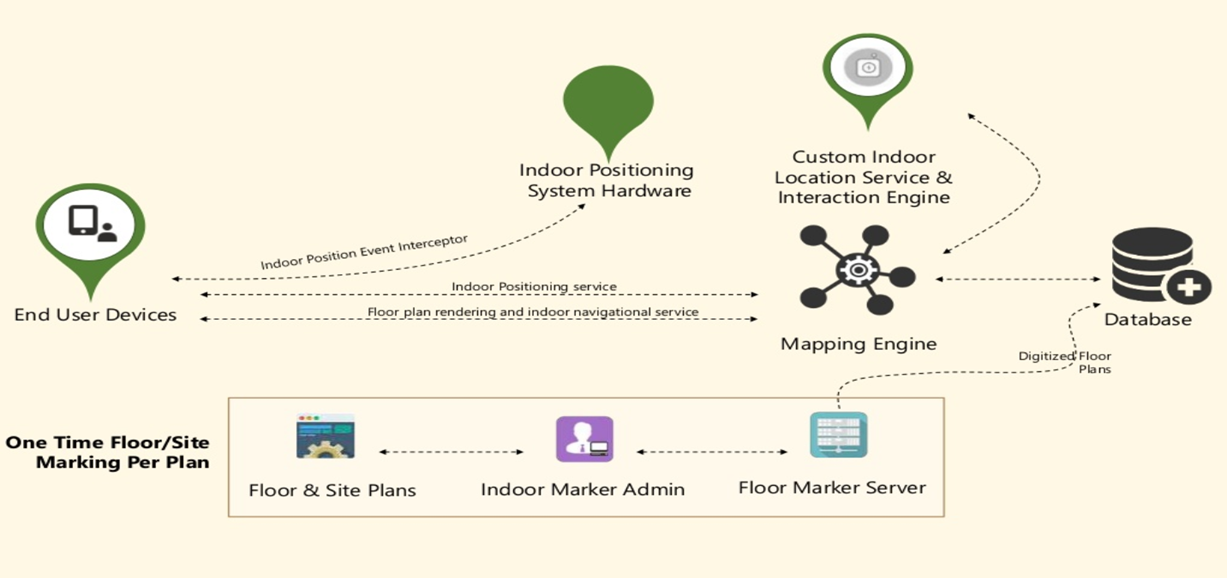
\includegraphics[width = 6in]{2.png}
    \caption{Workflow}
    \label{fig: blockbit}
\end{figure}
\begin{enumerate}
	\item 	Bottom most part of the diagram works as a mapping layer , this includes the floor plan of the premises which are used by the admin and stored in a database with the help of servers.
	\item 	As soon as End user enters the circumference of the beacon a trigger is fired and an URL is sent to the user.
	\item 	Clicking onto the URL takes the user to the web-app.
	\item 	Position detected is first sent to the database via mapper.
	\item 	Now users have to enter the destination.
	\item 	Once done it is also sent to the database 
	\item 	Both the starting and ending position along with all possible paths are sent to interaction engine where A* algorithm works.And the most optimised path is sent back to End user device.
\end{enumerate}

\newpage
\begin{center}
	\section{Applications of Indoor Navigation}
\end{center}
\subsection{Application}
As the name suggests, its main application is finding the positioning of the user and then navigating him/her to the desired destination.
\linebreak
Other Applications includes following :
\begin{itemize}
	\item {Indoor Marker Admin} Allows Admin to Locate  paths and points of interest.
	\item {Share Location} This feature will share your current location in building to other contact.
	\item {Emergency Evacuation} 	It finds the closest Emergency exit during a crisis.
	\item {Find a Friend}A friend gets a notification if other is in same locality.
	\item {Location Based Features}Provides Indoor Local Information
\end{itemize}

\subsection{Advantages}
\begin{itemize}
	\item This application can be used online as well as offline. So, internet connection is not a mandatory aspect.
	\item No need to install an application,it is a web-app as soon as the user enters the premises an URL will be sent.
	\item There is no need to enter the starting point manually. Users’ location will be fetched automatically.
	\item Fastest and Shortest path is provided in this application.
	\item Admin panel is provided for the owner of the premises, in order to enter the floorplan of the location and is also responsible for plotting points of features and possible paths .
	\item During any emergency, the application provides users with paths to emergency exit.
	\item It also provides a feature to find a friend. It gives a path from user to the friend if the friend is present in the same campus.
\end{itemize}

\subsection{Disadvantages}
\begin{itemize}
	\item The main drawback of this application is that it requires installation of multiple beacons in the campus.
	\item Maintenance of beacons is required. Every 5 to 8 years beacons’ batteries need to be changed.
	\item 	Also, if some floorplan is added into the premises, more beacons are needed to install.
	\item If the floorplan provided by the owner is not accurate than it may lead in detection of wrong position.

\end{itemize}

\newpage


\begin{center}
\section{CONCLUSION}
\end{center}
\par
Our indoor navigation system will consist of backend applications and client applications. Backend application will handle user authentication, persisting data and location data exchange between users. Client applications will be developed for Android and iOS mobile devices. It will provide functionalities of automatically locating users,navigating them to desired destinations via most optimised route, sharing their locations and showing their friends on indoor maps. 
\\

\newpage

%
%\bibliography{biblio}
\addcontentsline{toc}{section}{References}
\bibliographystyle{plain}

\begin{thebibliography}{21}
	\bibitem{paper1}“A Smart Indoor Navigation System over BLE”, 8th International Conference on Modern Circuits and Systems Technologies, 2019.
	
	\bibitem{paper2}“Time-Efficient Indoor Navigation and Evacuation with Fastest Path Planning Based on Internet of Things Technologies”, IEEE Transactions On Systems, Man, And Cybernetics : Systems, 2019.
	
	\bibitem{paper3}“Improved indoor position estimation algorithm based on geo-magnetism intensity “,International Conference on Indoor Positioning and Indoor Navigation, 2018.
	
	\bibitem{paper4}“BLE Beacons for Internet of Things Applications: Survey, Challenges and Opportunities”, IEEE Internet of Things Journal, Vol. A, No. B, 2018.
	
	\bibitem{paper5}“BLE Beacons for Internet of Things Applications: Survey, Challenges and Opportunities”, IEEE Internet of Things Journal, Vol. A, No. B, 2018.
	
	
	\bibitem{paper6}“Application of Augmented Reality in Campus Navigation ”, International Conference on Precision Machining, Non-Traditional Machining and Intelligent Manufacturing, 2019.
	
	
	\bibitem{paper7}“Indoor Navigation based on Linked Data at Honvéd Hospital, Budapest”, IEEE 12th International Symposium on Applied Computational Intelligence and Informatics ,SACI 2018
	
	\bibitem{paper8}“Indoor Navigation Using A* Algorithm” ,Springer International Publishing AG 2017 T. Herawan et al. (eds.), 2018
	
	
	\bibitem{paper9}“Using A* algorithm to find shortest path in Indoor positioning system”,International Research Journal of Engineering and Technology (IRJET), June -2018
	
\end{thebibliography}

\end{document}
